\documentclass[a4paper]{article}

\usepackage[portuguese]{babel}
\usepackage[utf8]{inputenc}
\usepackage{indentfirst}
\usepackage{graphicx}
\usepackage{verbatim}
\usepackage[margin=0.8in]{geometry}
\usepackage{amsmath}
\usepackage{listings}
\lstset{language=Prolog}  

\begin{document}

\setlength{\textwidth}{16cm}
\setlength{\textheight}{22cm}

\title{\Huge\textbf{Sixteen Stone}\linebreak\linebreak\linebreak
\Large\textbf{Relatório Intercalar}\linebreak\linebreak
\linebreak\linebreak

\includegraphics[scale=0.1]{images/feup-logo.png}\linebreak\linebreak
\linebreak\linebreak
\Large{Mestrado Integrado em Engenharia Informática e Computação} \linebreak\linebreak
\Large{Programação em Lógica}\linebreak
}

\author{\textbf{Grupo Sixteen\_Stone\_3:}\\
Diogo Filipe Costa - ei11014 \\
Maria Teresa Chaves - up201306842 \\
\linebreak\linebreak \\
 \\ Faculdade de Engenharia da Universidade do Porto \\ Rua Roberto Frias, s\/n, 4200-465 Porto, Portugal \linebreak\linebreak\linebreak
\linebreak\linebreak\vspace{1cm}}
\date{Novembro 2015}

\maketitle
\thispagestyle{empty}

%************************************************************************************************
%************************************************************************************************

\newpage

\section*{Resumo}

Nesta disciplina foi-nos proposto desenvolver um jogo de tabuleiro utilizando uma linguagem de programação em lógica, \textit{Prolog}. O nosso projeto incide sobre o jogo \textit{Sixteen Stones}. A aplicação que desenvolvemos centra-se na representação do tabuleiro de jogo quadrado, composto por células que serão ocupadas pelas pedras dos dois jogadores (Humano/Humano, Humano/Computador ou Computador/Computador) e movimentos que cada jogador poderá realizar.

Os resultados deste trabalho foram uma aplicação baseada no jogo \textit{Sixteen Stones}, fornecendo ao utilizador uma interface em modo texto. No modo Computador/Computador utilizamos inteligência artificial de forma a que, dependendo do nível de dificuldade escolhido, as jogadas fossem o mais parecidas com as jogadas que um ser humano faria.

\newpage

\tableofcontents

%************************************************************************************************
%************************************************************************************************

%*************************************************************************************************
%************************************************************************************************

\newpage

%%%%%%%%%%%%%%%%%%%%%%%%%%
\section{Introdução}

Pretende-se neste trabalho implementar, em linguagem Prolog, um jogo de tabuleiro para dois jogadores. Um jogo de tabuleiro caracteriza-se pelo tipo de tabuleiro e de peças, pelas regras de movimentação das peças (jogadas possíveis) e pelas condições de terminação do jogo com derrota, vitória ou empate. Pretende-se desenvolver uma aplicação para jogar um jogo deste tipo, usando o Prolog como linguagem de implementação. O jogo deve permitir três modos de utilização: Humano/Humano, Humano/Computador e Computador/Computador. Devem ser incluídos pelo menos dois níveis de jogo para o computador. Deve ser construída uma interface adequada com o utilizador, em modo de texto.
A aplicação terá um visualizador gráfico 3D, a realizar na

Descrever os objetivos e motivação do trabalho. Descrever num parágrafo breve a estrutura do relatório.


%%%%%%%%%%%%%%%%%%%%%%%%%%
\section{O Jogo Sixteen Stones}

Sixteen Stone é o nome de um jogo de tabuleiro abstrato de forma quadrada, jogado normalmente num tabuleiro de 5x5 (pode ter outras dimensões), para dois jogadores. Inicialmente, cada jogador tem 8 pedras vermelhas ou azuis (tabuleiro 5x5), colocando-as de forma alternada em qualquer uma das células livres, sendo que o jogador vermelho é o primeiro a jogar. Assim que todas as pedras estejam no tabuleiro, o jogo começa. 

O jogador vermelho começa a jogar e alterna de turno com o jogador adversário. Um jogador pode no seu respetivo turno realizar cada uma das seguintes jogadas: \textit{Push}, \textit{Move} e \textit{Sacrifice}. No primeiro turno de cada jogador, deve ser feito um \textit{Push} ou um \textit{Move}, mas nunca ambos. \\

\textbf{Push}\\

Para realizar um  \textit{Push} é necessário que o jogador tenha mais pedras nessa linha que o adversário. Assim, se após um  \textit{Push}, a pedra do adversário é "empurrada" para fora do tabuleiro, então vai para o "banco" do respetivo jogador. As pedras que são "empurradas" apenas se movem uma célula na direção do \textit{Push}, que pode ser realizado em qualquer direção. O número de pedras máximo (PE) que um jogador pode "empurrar" é igual a:

Um jogador não pode realizar um  \textit{Push} nas suas próprias pedras. 
Por fim, para realizar um \textit{Push} é necessário que exista uma pedra para ser "empurrada".

\begin{equation}
	PE = P - 1 \text{\hspace{7mm}(sendo P o número das suas pedras nessa linha)}
\end{equation}

\begin{figure}[!htb]
\minipage{0.5\textwidth}
	\centering
  	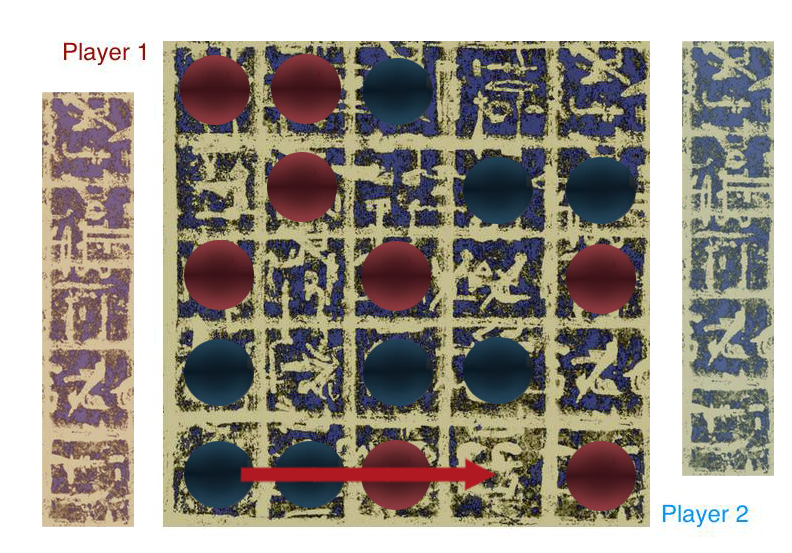
\includegraphics[scale=0.2]{images/push_not_pool.png}
	\caption{\textit{Push} sem que a pedra adversária seja "empurrada" para fora do tabuleiro.}
\endminipage\hfill
\minipage{0.5\textwidth}
 \vspace*{2.3cm}
	\centering
	 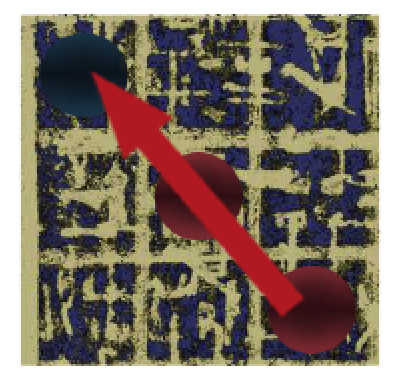
\includegraphics[scale=0.2]{images/push_pool.png} \vspace*{0.3cm}
	\caption{\textit{Push} em que a pedra do adversário é "empurrada" para fora do tabuleiro.}
\endminipage
\end{figure}

\newpage

\begin{figure}[!htb]
	\centering
	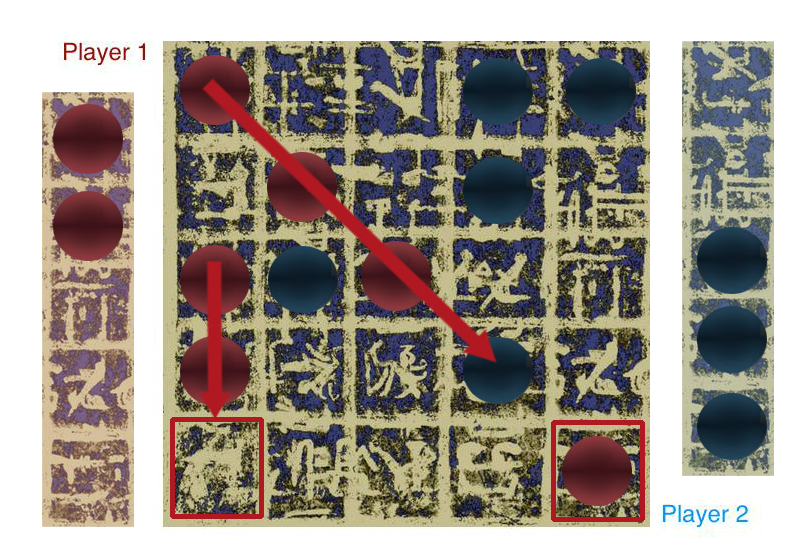
\includegraphics[scale=0.2]{images/invalid_push.png} 
	\caption{Push inválido: nas suas próprias pedras (a); numa célula vazia (b).}
\end{figure}

\textbf{Move}\\

É possível realizar um  \textit{Move} para uma célula vazia em qualquer direção. Se o jogador tentar realizar um \textit{Move} para uma célula ocupada, então é considerado uma jogada inválida.

Se um jogador realizar um \textit{Move} e a sua pedra ficar voluntariamente cercada, esta não é capturada.

\begin{figure}[!htb]
\minipage{0.5\textwidth}
	\centering
  	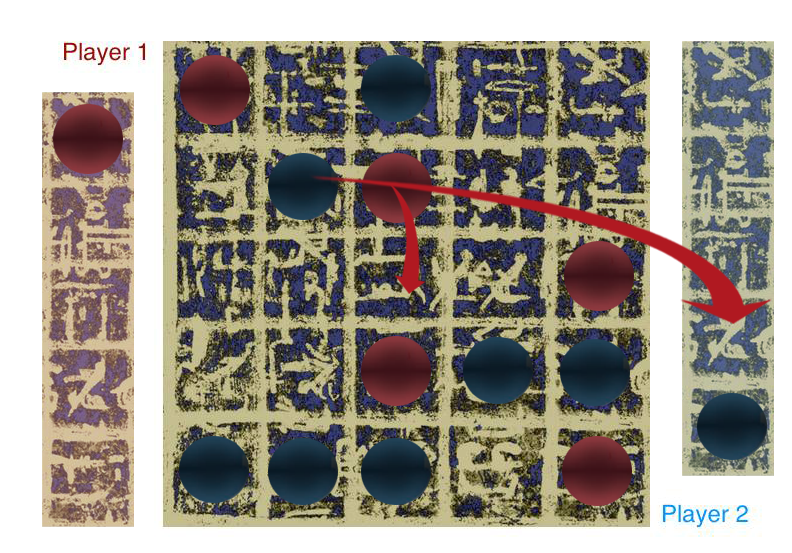
\includegraphics[scale=0.3]{images/move_cap.png} 
	\caption{Pedra azul capturada após um \textit{Move} de uma pedra vermelha.}
\endminipage\hfill
\minipage{0.5\textwidth}
	\vspace*{3.1cm}
	\centering
	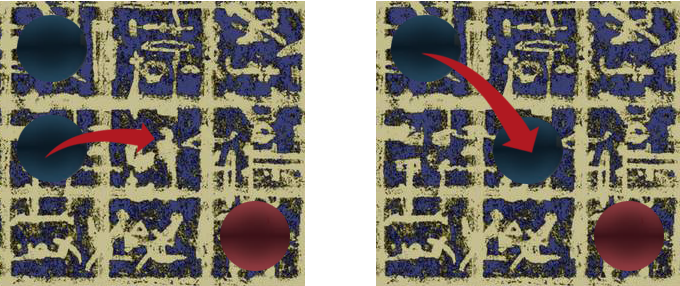
\includegraphics[scale=0.2]{images/valid_invalid_move.png} \vspace*{0.3cm}
	\caption{\textit{Move} válido (a) e um \textit{Move} inválido (b).}
\endminipage
\end{figure}

\textbf{Sacrifice}\\

Um jogador pode sacrificar uma pedra do seu "banco", permanentemente, para poder realizar um \textit{Push} ou um \textit{Move} adicional.\\

% falta imagem para o sacrifice...

\textbf{Capture}\\

Uma pedra fica cercada quando existem pelo menos em duas direções opostas pedras adversárias. Por exemplo se após um \textit{Move} se alguma das pedras adversárias ficar cercada, então esta é capturada e substituída por uma pedra do "banco" do jogador que a capturou.

Após um \textit{Push}, se uma das pedras do jogador atual se move para uma posição que já esta ocupada por uma das suas pedras e fica a cercar uma pedra adversária então é capturada.

Se após um \textit{Push} uma das pedras do adversário fica cercada, então é capturada.

Quando uma pedra adversária é capturada, esta pedra é colocada na \textit{Pool} do adversário e é substituída por outra da \textit{Pool} do jogador que efetuou a jogada.

\begin{figure}[!htb]
	\centering
	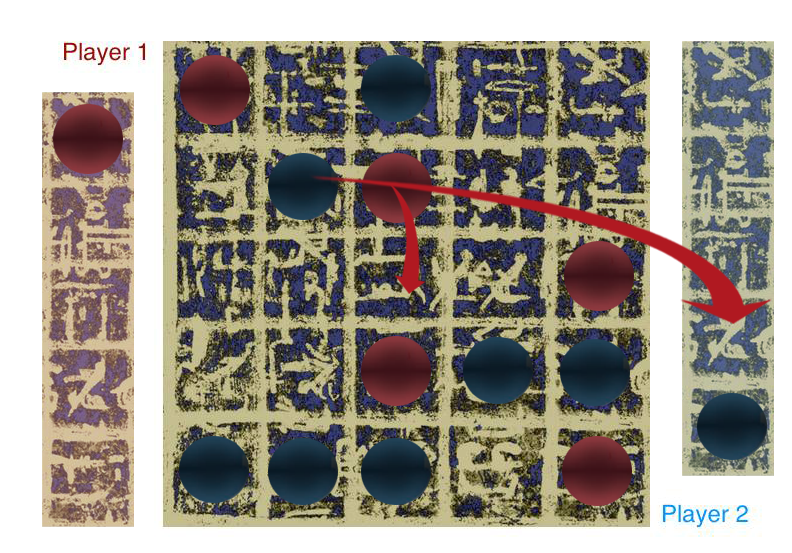
\includegraphics[scale=0.3]{images/move_cap.png} 
	\caption{Pedra azul capturada após um \textit{Move} de uma pedra vermelha.} %melhorar imagem...
\end{figure}

O jogo termina quando o jogador vencedor consegue reduzir para um o número de pedras em jogo do adversário.

%%%%%%%%%%%%%%%%%%%%%%%%%%
\section{Lógica do Jogo}

Descrever o projeto e implementação da lógica do jogo em Prolog, incluindo a forma de representação do estado do tabuleiro e sua visualização, execução de movimentos, verificação do cumprimento das regras do jogo, determinação do final do jogo e cálculo das jogadas a realizar pelo computador utilizando diversos níveis de jogo. Sugere-se a estruturação desta secção da seguinte forma:

\subsection{Representação do Estado do Jogo}

O tabuleiro é representado por uma lista de listas  $L = \{L_1, L_2, ... , L_n\} , n > 0  \wedge n$ é múltiplo de $5$, em que $n$ é a dimensão do tabuleiro. \par
Com o predicado \texttt{make\_board} é possível criar um tabuleiro (\textit{Board}) com um tamanho \textit{Size}. Para isso o \texttt{make\_board} utiliza o predicado \texttt{make\_line} para criar uma linha e depois usa o \texttt{make\_board} recursivamente. De forma a tornar mais clara a visualização do tabuleiro de jogo, após criá-lo com o \texttt{make\_board} utiliza-se o predicado \texttt{print\_board} que o imprime no ecrã.

\begin{figure}[!htb]
	\centering
	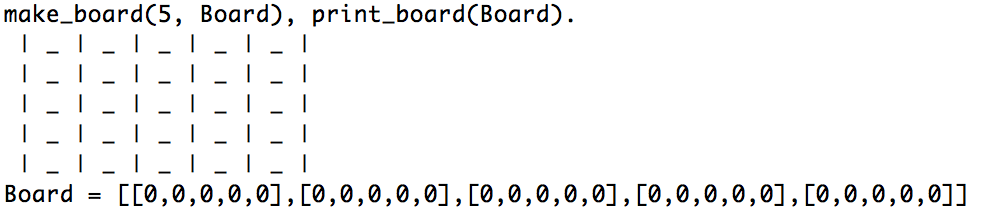
\includegraphics[scale=0.45]{images/make_board.png}
	\caption{Estado inicial do jogo.}
\end{figure}

A figura acima demonstra o estado do tabuleiro na sua fase inicial, sem nenhuma célula preenchida. De uma forma mais visual, segue-se abaixo uma figura demonstrativa do tabuleiro.

\begin{figure}[!htb]
	\centering
	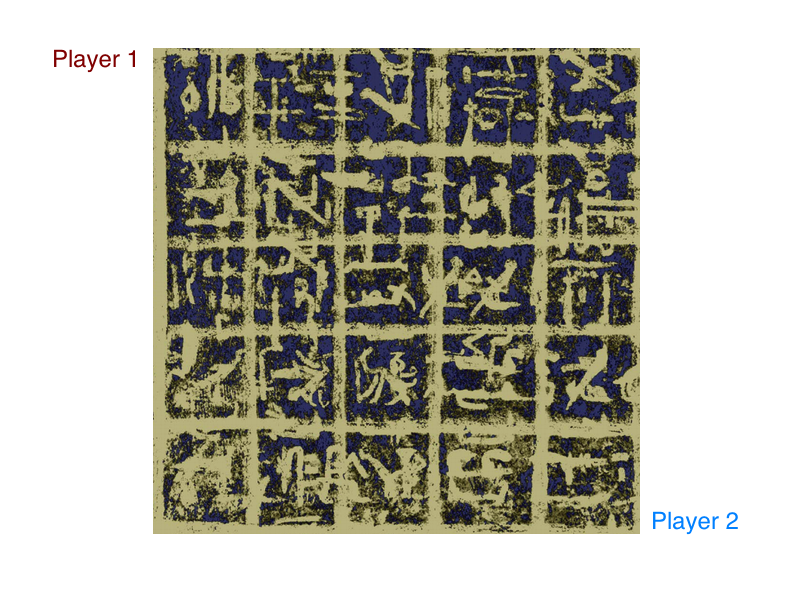
\includegraphics[scale=0.3]{images/board.png}
	\caption{Tabuleiro de jogo.}
\end{figure}

O jogador pode realizar cada uma das três jogadas possíveis: \textit{Push}, \textit{Move} e \textit{Sacrifice}. Para o \textit{Push} é usado o predicado \texttt{push(Stone\_src, Stone\_dst, Dir, Board)}, onde \texttt{Stone\_src} e \texttt{Stone\_dst} são as coordenadas x-y (separadas por um traço) das pedras inicial e destino, \texttt{Dir} é a direção do \textit{Push} e pode ter os valores: 0 (cima), 1 (direita), 2 (baixo) ou 3 (esquerda) e \texttt{Board} é o tabuleiro que é retornado após o \textit{Push}.

\begin{figure}[!htb]
	\centering
	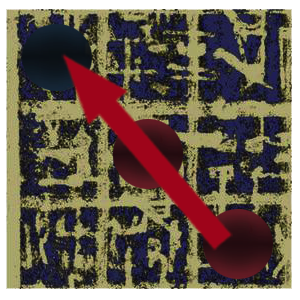
\includegraphics[scale=0.2]{images/push.png}
	\caption{Exemplo de um \textit{Push}.}
\end{figure}

\newpage

Para o \textit{Move} é usado o predicado \texttt{move(Stone\_src, Cell\_dst, Board)}, onde \texttt{Stone\_src} é a pedra que se pretende mover, \texttt{Cell\_dst} é a célula de destino e o \texttt{Board} é o tabuleiro que é retornado.

\begin{figure}[!htb]
	\centering
	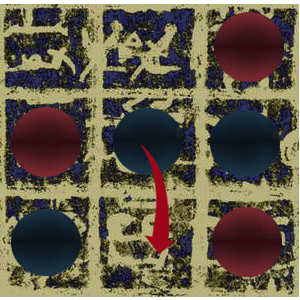
\includegraphics[scale=0.3]{images/move.png}
	\caption{Exemplo de um \textit{Move}.}
\end{figure}

Para o \textit{Sacrifice} é usado o predicado \texttt{sacrifice(Stone, Board)}, onde \texttt{Stone} é a pedra que se pretende sacrificar e o \texttt{Board} é o tabuleiro que é retornado.

\begin{figure}[!htb]
	\centering
	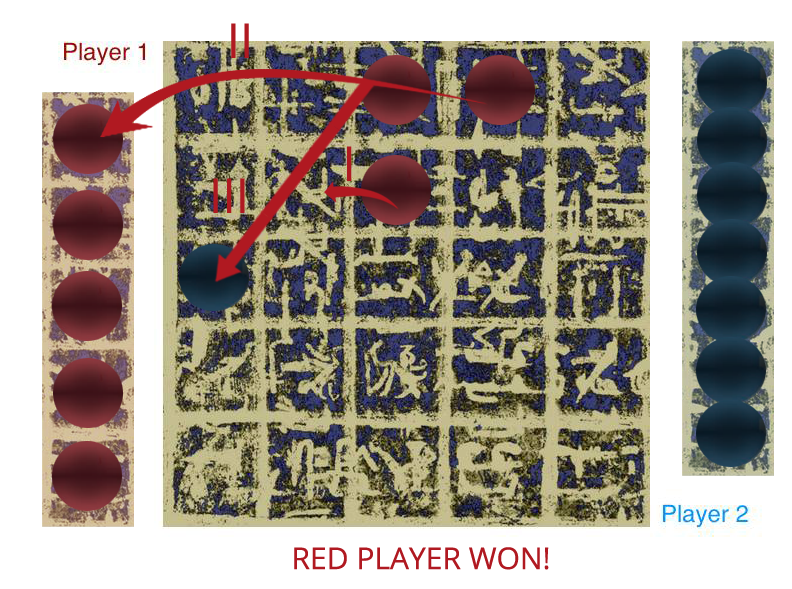
\includegraphics[scale=0.3]{images/sacrifice.png}
	\caption{Exemplo de um \textit{Sacrifice} (II).}
\end{figure}

Existe ainda um predicado \texttt{moveToPool(Stone, Player, Pool)} que move uma uma pedra (\texttt{Stone}) para o "banco" de um dado jogador (\texttt{Player}) retorna o "banco" do jogador (\texttt{Pool}) após a pedra ter sido movida.

\begin{figure}[!htb]
	\centering
	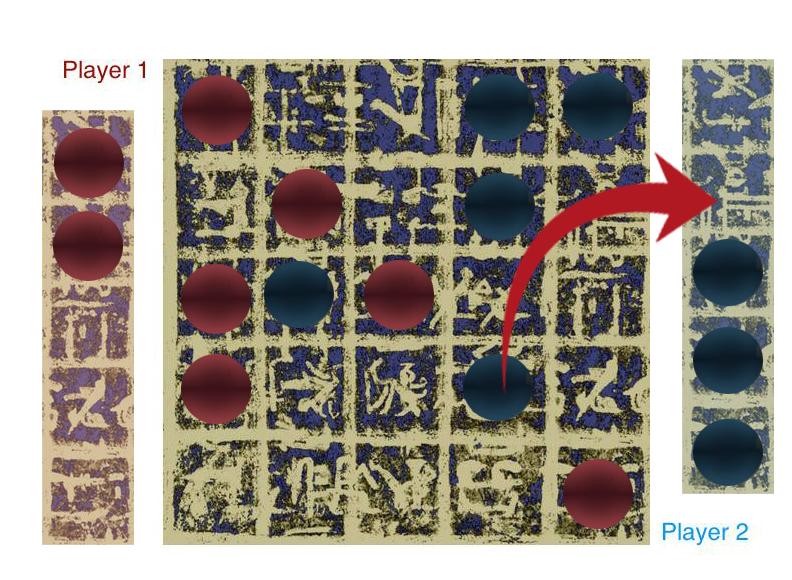
\includegraphics[scale=0.2]{images/pool.png}
	\caption{Exemplo de uma pedra a ser colocada no "banco" de um jogador.}
\end{figure}

%----------------------------------------------------------------------------------------------------------------------------------------------------------------------
\section{Visualização do Tabuleiro}

A cor das pedras dos jogadores são representadas pelos carateres \texttt{x} para as pedras azuis e \texttt{o} para as pedras vermelhas, sendo que o carater \texttt{\_} é usado para representar casas vazias.

Os predicados utilizados para construir e visualizar o tabuleiro são:

\begin{itemize}
	\item \texttt{make\_line/2} - Gera uma linha do tabuleiro
	\item \texttt{make\_board/2} - Gera um tabuleiro de jogo com o tamanho especificado
	\item \texttt{print\_line/1} - Predicado para imprimir uma linha do tabuleiro
	\item \texttt{print\_board/1} - Predicado que imprime o tabuleiro, passado sob a forma de uma lista de listas
	\item \texttt{draw\_board/2} - Predicado que chama os predicados anteriores para gerar um tabuleiro com um tamanho especificado e imprime-o no ecrã
\end{itemize}

\begin{figure}[!htb]
	\centering
	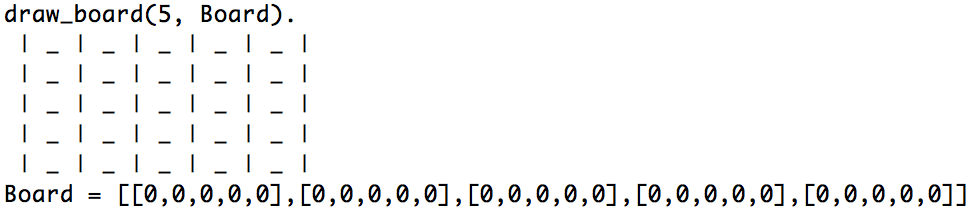
\includegraphics[scale=0.6]{images/draw_board.png}
	\caption{Exemplo de chamada do predicado \texttt{draw\_board} para um tamanho de 5x5}
\end{figure}

Numa fase já intermédia do jogo, o tabuleiro poderá atingir um ponto com o seguinte o formato:

\begin{figure}[!htb]
	\centering
	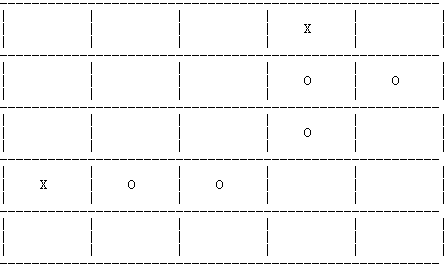
\includegraphics[scale=0.5]{images/board_prolog.png}
	\caption{Exemplo de fase intermédia do jogo.}
\end{figure}

De uma forma mais visual, segue-se abaixo uma figura ilustrativa da fase respetiva do tabuleiro.

\begin{figure}[!htb]
	\centering
	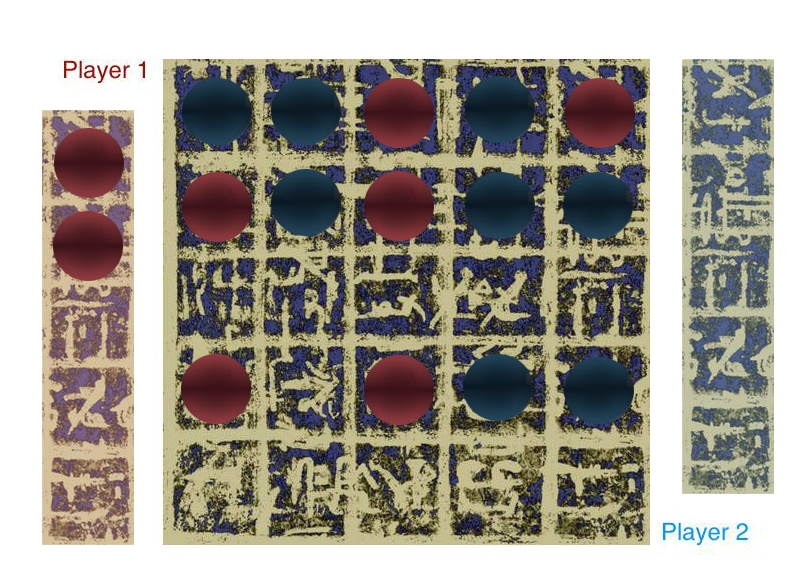
\includegraphics[scale=0.6]{images/board_inter.png}
	\caption{Forma mais visual de uma fase intermédia do jogo.}
\end{figure}

\newpage

%----------------------------------------------------------------------------------------------------------------------------------------------------------------------

\subsection{Lista de Jogadas Válidas} Obtenção de uma lista de jogadas possíveis. Exemplo: \textit{valid\_moves(+Board, -ListOfMoves)}.

\subsection{Execução de Jogadas} Validação e execução de uma jogada num tabuleiro, obtendo o novo estado do jogo. Exemplo: \textit{move(+Move, +Board, -NewBoard)}.

\subsection{Avaliação do Tabuleiro} Avaliação do estado do jogo, que permitirá comparar a aplicação das diversas jogadas disponíveis. Exemplo: \textit{value(+Board, +Player, -Value)}.

\subsection{Final do Jogo} Verificação do fim do jogo, com identificação do vencedor. Exemplo: \textit{game\_over(+Board, -Winner)}.

\subsection{Jogada do Computador} Escolha da jogada a efetuar pelo computador, dependendo do nível de dificuldade. Por exemplo: \textit{choose\_move(+Level, +Board, -Move)}.


%%%%%%%%%%%%%%%%%%%%%%%%%%
\section{Interface com o Utilizador}

Descrever o módulo de interface com o utilizador em modo de texto.


%%%%%%%%%%%%%%%%%%%%%%%%%%
\section{Conclusões}
Que conclui deste projecto? Como poderia melhorar o trabalho desenvolvido?


\clearpage
\addcontentsline{toc}{section}{Bibliografia}
\renewcommand\refname{Bibliografia}
\bibliographystyle{plain}
\bibliography{myrefs}

\newpage
\appendix
\section{Nome do Anexo}
Código Prolog implementado devidamente comentado e outros elementos úteis que não sejam essenciais ao relatório.

\end{document}
